En lo que resta de esta sección nos ocuparemos de relacionar parejas de grafos mediante funciones.
\begin{Def}\label{Def:homomorfismo}
   Sean $G=(V,E)$ y $G'=(V',E')$ dos grafos. Decimos que $\varphi:V\to V'$ es un homomorfismo de $G$ en $G'$ si $\left\lbrace u,v\right\rbrace\in E$ implica $\left\lbrace \varphi(u),\varphi(v) \right\rbrace\in E'$ para cualesquiera vértices $u,v\in V$.
\end{Def}
El hecho de que $\left\lbrace u,v \right\rbrace\in E$ implique $\left\lbrace \varphi(u),\varphi(v)\right\rbrace\in E'$ lo resumimos diciendo que $\varphi$ preserva la adyacencia entre vértices, puesto que $\varphi$ envía vértices adyacentes de $G$ a vértices adyacentes de $G'$.
\begin{Ejm}\label{Ejm:homomorfismos}
   La función
   \begin{center}
   $\hfill
   \begin{array}{rcl}
      \varphi_1 \colon V(G) &\to& V(G') \\
      v_1 &\mapsto& w_1 \\
      v_2 &\mapsto& w_2 \\
      v_3 &\mapsto& w_3 \\
      v_4 &\mapsto& w_2 \\
      v_5 &\mapsto& w_1
   \end{array}
   \hfill$
   \end{center}
   es un homomorfismo de $G$ en $G'$, donde $G$ y $G'$ son los grafos que se muestran a continuación.
   \begin{figure}[H]
  \centering
  % Primer grafo (G_1)
  \begin{minipage}[t]{0.49\textwidth}
    \centering
    \scalebox{0.7}{% Ajusta este valor (ej. 0.6, 0.7, 0.8) para controlar el tamaño
      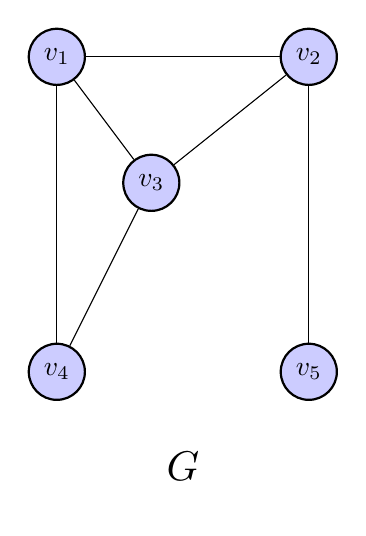
\begin{tikzpicture}[scale=.8,auto=left,every node/.style={circle,fill=blue!20,draw=black,thick}]
  % Vértices G1
  \node (n1) at (0, 4) {$v_1$};
  \node (n2) at (4, 4) {$v_2$};
  \node (n3) at (1.5, 2) {$v_3$};
  \node (n4) at (0, -1) {$v_4$};
  \node (n5) at (4, -1) {$v_5$};

  % Aristas G1 (Quitando n2/n4)
  \foreach \from/\to in {n1/n2, n1/n3, n1/n4, n2/n3, n2/n5, n3/n4}
    \draw (\from) -- (\to);

  % Título
  \node[draw=none, fill=none, scale=1.5] at (2, -2.5) {$G$};
\end{tikzpicture}

    }
  \end{minipage}%
  \hspace{-2em}%
  % Segundo grafo (G'_1)
  \begin{minipage}[t]{0.49\textwidth}
    \centering
    \scalebox{0.7}{% Usa el mismo factor de escala para que guarden proporción
      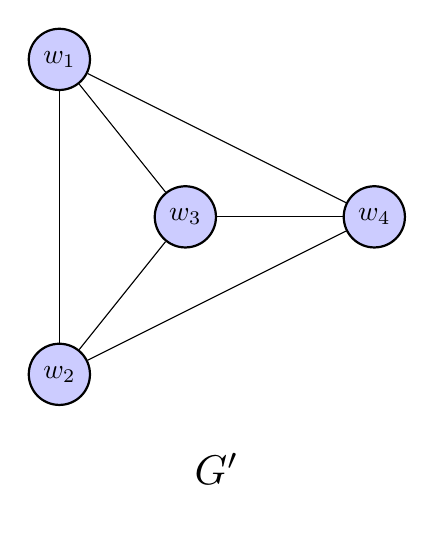
\begin{tikzpicture}[scale=.8,auto=left,every node/.style={circle,fill=blue!20,draw=black,thick}]
  % Vértices G'1
  \node (m1) at (0, 4) {$w_1$};
  \node (m2) at (0, -1) {$w_2$};
  \node (m3) at (2, 1.5) {$w_3$};
  \node (m4) at (5, 1.5) {$w_4$};

  % Aristas G'1
  \foreach \from/\to in {m1/m2, m1/m3, m1/m4, m2/m3, m2/m4, m3/m4}
    \draw (\from) -- (\to);

  % Título
  \node[draw=none, fill=none, scale=1.5] at (2.5, -2.5) {$G'$};
\end{tikzpicture}

    }
  \end{minipage}
  
  \caption{$\varphi$ es un homomorfismo de $G_1$ en $G'_1$}
  \label{fig:homomorfismo_grafos}
\end{figure}

   Para verificar que $\varphi_1$ es un homomorfismo notemos que $\varphi_1$ preserva la adyacencia entre vértices de $G$:
   \begin{center}
   $\hfill
   \begin{array}{rcl}
      \{v_1, v_2\} \in E(G) &\text{ y }& \{\varphi_1(v_1), \varphi_1(v_2)\} = \{w_1, w_2\} \in E(G'), \\
      \{v_1, v_3\} \in E(G) &\text{ y }& \{\varphi_1(v_1), \varphi_1(v_3)\} = \{w_1, w_3\} \in E(G'), \\
      \{v_1, v_4\} \in E(G) &\text{ y }& \{\varphi_1(v_1), \varphi_1(v_4)\} = \{w_1, w_2\} \in E(G'), \\
      \{v_2, v_3\} \in E(G) &\text{ y }& \{\varphi_1(v_2), \varphi_1(v_3)\} = \{w_2, w_3\} \in E(G'), \\
      \{v_2, v_5\} \in E(G) &\text{ y }& \{\varphi_1(v_2), \varphi_1(v_5)\} = \{w_2, w_1\} \in E(G'), \\
      \{v_3, v_4\} \in E(G) &\text{ y }& \{\varphi_1(v_3), \varphi_1(v_4)\} = \{w_3, w_2\} \in E(G').
   \end{array}
   \hfill$
   \end{center}
   En cambio la función
   \begin{center}
   $\hfill
   \begin{array}{rcl}
      \varphi_2 \colon V(G) &\to& V(G') \\
      v_1 &\mapsto& w_4 \\
      v_2 &\mapsto& w_2 \\
      v_3 &\mapsto& w_4 \\
      v_4 &\mapsto& w_1 \\
      v_5 &\mapsto& w_3
   \end{array}
   \hfill$
   \end{center}
   no es un homomorfismo de $G$ en $G'$, pues $\left\lbrace v_1,v_3\right\rbrace\in E(G)$ pero $\left\lbrace \varphi(v_1),\varphi(v_3)\right\rbrace=\left\lbrace w_4\right\rbrace\notin E(G')$.\\
   Podemos ver también que la función
   \begin{center}
   $\hfill
   \begin{array}{rcl}
      \psi \colon V(H) &\to& V(H') \\
      x_1 &\mapsto& y_1 \\
      x_2 &\mapsto& y_2 \\
      x_3 &\mapsto& y_3 \\
      x_4 &\mapsto& y_4 
   \end{array}
   \hfill$
   \end{center}
   es un homomorfismo entre los grafos $H$ y $H'$, que se presentan en la \Cref{fig:homomorfismo_grafos_2}
   \begin{figure}[H]
  \centering
  % Primer grafo (G_1)
  \begin{minipage}[t]{0.49\textwidth}
    \centering
    \scalebox{0.7}{% Ajusta este valor (ej. 0.6, 0.7, 0.8) para controlar el tamaño
      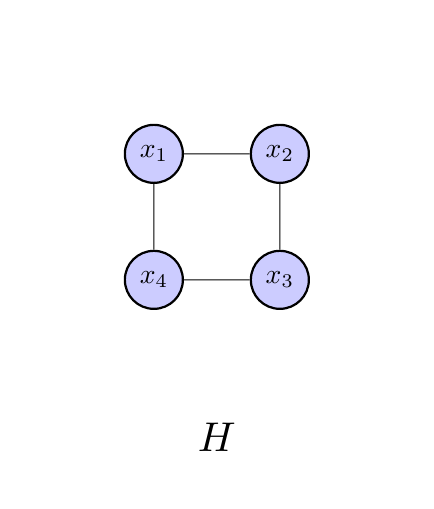
\begin{tikzpicture}[scale=.8,auto=left,every node/.style={circle,fill=blue!20,draw=black,thick}]
  % Vértices del cuadrado interior (C_4)
   \node (w1) at (-1, 1) {$x_1$};
  \node (w2) at (1, 1) {$x_2$};
  \node (w3) at (1, -1) {$x_3$};
  \node (w4) at (-1, -1) {$x_4$};

  % Vértices del cuadrado exterior (C_4 más grande)
  \node (w5) at (-2.5, 2.5) [opacity=0]{$w_5$};
  \node (w6) at (2.5, 2.5) [opacity=0]{$w_6$};
  \node (w7) at (2.5, -2.5) [opacity=0]{$w_7$};
  \node (w8) at (-2.5, -2.5) [opacity=0]{$w_8$};

  % Aristas del cuadrado interior
  \foreach \from/\to in {w1/w2, w2/w3, w3/w4, w4/w1}
    \draw (\from) -- (\to);

  % Título del grafo en la parte inferior
  \node[draw=none, fill=none, scale=1.5] at (0,-3.5) {$H$};
\end{tikzpicture}

    }
  \end{minipage}%
  \hspace{-3.5em}%
  % Segundo grafo (G'_1)
  \begin{minipage}[t]{0.49\textwidth}
    \centering
    \scalebox{0.7}{% Usa el mismo factor de escala para que guarden proporción
      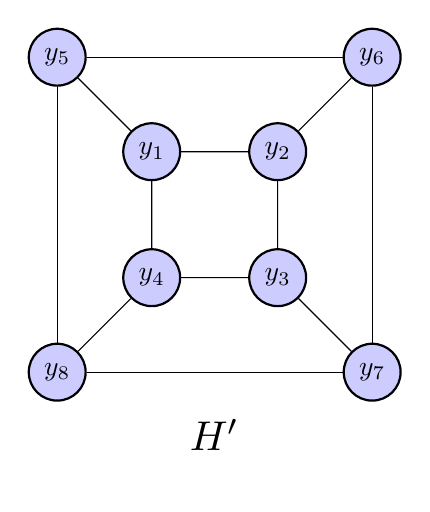
\begin{tikzpicture}[scale=.8,auto=left,every node/.style={circle,fill=blue!20,draw=black,thick}]
  % Vértices del cuadrado interior (C_4)
  \node (w1) at (-1, 1) {$y_1$};
  \node (w2) at (1, 1) {$y_2$};
  \node (w3) at (1, -1) {$y_3$};
  \node (w4) at (-1, -1) {$y_4$};

  % Vértices del cuadrado exterior (C_4 más grande)
  \node (w5) at (-2.5, 2.5) {$y_5$};
  \node (w6) at (2.5, 2.5) {$y_6$};
  \node (w7) at (2.5, -2.5) {$y_7$};
  \node (w8) at (-2.5, -2.5) {$y_8$};

  % Aristas del cuadrado interior
  \foreach \from/\to in {w1/w2, w2/w3, w3/w4, w4/w1}
    \draw (\from) -- (\to);

  % Aristas del cuadrado exterior
  \foreach \from/\to in {w5/w6, w6/w7, w7/w8, w8/w5}
    \draw (\from) -- (\to);

  % Conexiones entre los vértices correspondientes de ambos cuadrados
  \foreach \from/\to in {w1/w5, w2/w6, w3/w7, w4/w8}
    \draw (\from) -- (\to);

  % Título del grafo en la parte inferior
  \node[draw=none, fill=none, scale=1.5] at (0,-3.5) {$H'$};
\end{tikzpicture}

    }
  \end{minipage}
  
  \caption{$H$ y $H'$}
  \label{fig:homomorfismo_grafos_2}
\end{figure}

   pues
   \begin{center}
   $\hfill
   \begin{array}{rcl}
      \{x_1, x_2\} \in E(H) &\text{ y }& \{\varphi_1(x_1), \varphi_1(x_2)\} = \{y_1, y_2\} \in E(H'), \\
      \{x_2, x_3\} \in E(H) &\text{ y }& \{\varphi_1(x_2), \varphi_1(x_3)\} = \{y_2, y_3\} \in E(H'), \\
      \{x_3, x_4\} \in E(H) &\text{ y }& \{\varphi_1(x_3), \varphi_1(x_4)\} = \{y_3, y_4\} \in E(H'), \\
      \{x_4, x_1\} \in E(H) &\text{ y }& \{\varphi_1(x_4), \varphi_1(x_1)\} = \{y_4, y_1\} \in E(H').
   \end{array}
   \hfill$
   \end{center}
\end{Ejm}
Estamos interesados en encontrar funciones entre vértices que permitan determinar si los grafos en cuestión son ``indistinguibles'' para la teoría construida. Un homomorfismo no es suficiente para esto: notemos que en la \Cref{Def:homomorfismo}, un homomorfismo puede enviar vértices no adyacentes en el grafo de partida a vértices adyacentes en el grafo de llegada. Como muestra de esto, en el \Cref{Ejm:homomorfismos}, se tiene que $\varphi_1$ es un homomorfismo de $G$ en $G'$, y a pesar de que $v_3$ y $v_5$ no son adyacentes en $G$, vemos que $\varphi_1(v_3)=w_3$ y $\varphi_1(v_5)=w_1$ sí son adyacentes en $G'$. Un primer paso sería exigir que la función, además de preservar la adyacencia de los vértices del grafo de partida, no envíe vértices no adyacentes en vértices adyacentes. Sin embargo, esta propiedad la cumple la función $\psi$ del \Cref{Ejm:homomorfismos}, conectando al grafo $H$ de $4$ vértices y $4$ aristas con el grafo $H'$ de $8$ vértices y $12$ aristas. Incluir la exigencia de que la función sea biyectiva solventa el problema y se obtiene la definición de \textit{isomorfismo} entre grafos.
\begin{Def}
   Sean $G=(V,E)$ y $G'=(V',E')$ dos grafos. Decimos que una función $\varphi:V\to V'$ es un \textbf{isomorfismo} de $G$ en $G'$ si $\varphi$ es biyectiva y $\left\lbrace u,v\right\rbrace\in E$, si y sólo si, $\left\lbrace \varphi(u), \varphi(v)\right\rbrace\in E'$, para cualesquiera vértices $u,v\in V$. Si existe un isomorfismo de $G$ en $G'$ decimos que $G$ y $G'$ son \textbf{isomorfos} y escribimos $G\simeq G'$. Un isomorfismo de $G$ en sí mismo es llamado un \textbf{automorfismo} de $G$.
\end{Def}
Usualmente no hacemos distinción alguna entre grafos isomorfos. Esto es lo que nos permite hablar de ``\textit{el} camino de $6$ vértices'', ``\textit{el} grafo completo de $4$ vértices'', etc.
\begin{Obs}
   En cualquier grafo $G$ la función identidad de $V(G)$ es un automorfismo de $G$.
\end{Obs}
\begin{Ejm}
   En la \Cref{fig:primer_isomorfismo} los grafos $G$ y $G'$ son isomorfos. 
   \begin{figure}[H]
  \centering
  % Primer grafo (G_1)
  \begin{minipage}[t]{0.49\textwidth}
    \centering
    \scalebox{0.7}{% Ajusta este valor (ej. 0.6, 0.7, 0.8) para controlar el tamaño
      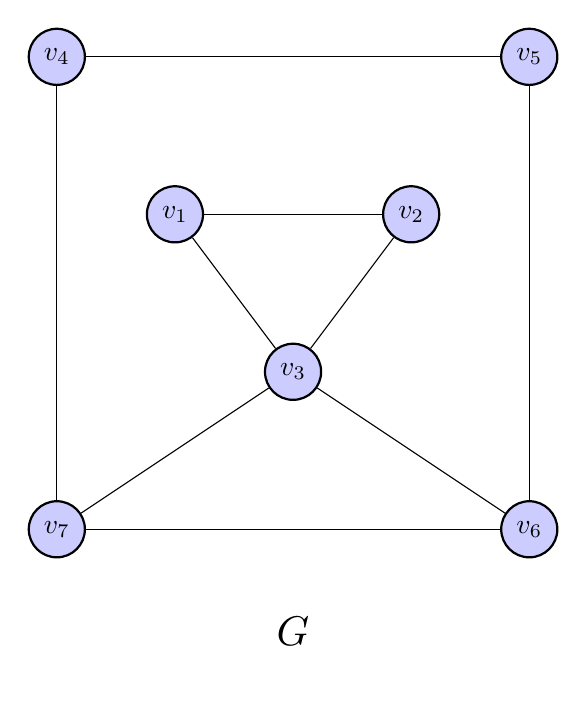
\begin{tikzpicture}[auto=left,every node/.style={circle,fill=blue!20,draw=black,thick}]
  % Cuadrado exterior (v4 y v5 en la parte superior; v7 y v6 en la parte inferior)
  \node (v4) at (-3, 3.5) {$v_4$};
  \node (v5) at (3, 3.5) {$v_5$};
  \node (v6) at (3, -2.5) {$v_6$};
  \node (v7) at (-3, -2.5) {$v_7$};

  % Triángulo interior (v1, v2, v3)
  \node (v1) at (-1.5, 1.5) {$v_1$};
  \node (v2) at (1.5, 1.5) {$v_2$};
  \node (v3) at (0, -0.5) {$v_3$};

  % Aristas del cuadrado exterior
  \foreach \from/\to in {v4/v5, v5/v6, v6/v7, v7/v4}
    \draw (\from) -- (\to);

  % Aristas del triángulo interior
  \foreach \from/\to in {v1/v2, v2/v3, v3/v1}
    \draw (\from) -- (\to);

  % Conexiones del vértice inferior v3 a las esquinas inferiores
  \draw (v3) -- (v7);
  \draw (v3) -- (v6);

  % Título
  \node[draw=none, fill=none, scale=1.5] at (0,-3.8) {$G$};
\end{tikzpicture}

    }
  \end{minipage}%
  \hspace{-3em}%
  % Segundo grafo (G'_1)
  \begin{minipage}[t]{0.49\textwidth}
    \centering
    \scalebox{0.7}{% Usa el mismo factor de escala para que guarden proporción
      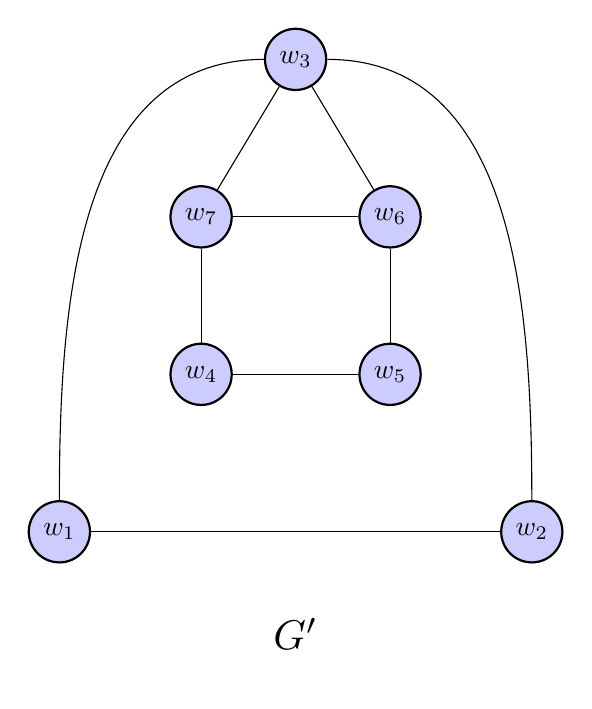
\begin{tikzpicture}[auto=left,every node/.style={circle,fill=blue!20,draw=black,thick}]
  % Vértice superior en la misma cota máxima (y=3.5)
  \node (w3) at (0, 3.5) {$w_3$};

  % "Casa" interior (w7, w6, w5, w4)
  \node (w7) at (-1.2, 1.5) {$w_7$};
  \node (w6) at (1.2, 1.5) {$w_6$};
  \node (w5) at (1.2, -0.5) {$w_5$};
  \node (w4) at (-1.2, -0.5) {$w_4$};

  % Vértices inferiores en la misma cota mínima (y=-2.5)
  \node (w1) at (-3, -2.5) {$w_1$};
  \node (w2) at (3, -2.5) {$w_2$};

  % Aristas de la estructura interior
  \foreach \from/\to in {w7/w6, w6/w5, w5/w4, w4/w7, w3/w7, w3/w6}
    \draw (\from) -- (\to);

  % Arista de la base exterior
  \draw (w1) -- (w2);

  % Arcos exteriores curvados
  \draw (w3) to[out=180, in=90] (w1);
  \draw (w3) to[out=0, in=90] (w2);

  % Título
  \node[draw=none, fill=none, scale=1.5] at (0,-3.8) {$G'$};
\end{tikzpicture}

    }
  \end{minipage}
  
  \caption{$\psi$ es un homomorfismo de $H$ en $H'$}
  \label{fig:homomorfismo_grafos_2}
\end{figure}

   Consideremos la función $\varphi:V(G)\to V(G'):v_i\mapsto w_i$ para $i=1,2,\dots ,7$. Se tiene que $\varphi$ es biyectiva. Además
   \begin{center}
   $\hfill
   \begin{array}{rcl}
      \{v_1, v_2\} \in E(G) &\text{ y }& \{\varphi(v_1), \varphi(v_2)\} = \{w_1, w_2\} \in E(G'), \\
      \{v_1, v_3\} \in E(G) &\text{ y }& \{\varphi(v_1), \varphi(v_3)\} = \{w_1, w_3\} \in E(G'), \\
      \{v_2, v_3\} \in E(G) &\text{ y }& \{\varphi(v_2), \varphi(v_3)\} = \{w_2, w_3\} \in E(G'), \\
      \{v_3, v_7\} \in E(G) &\text{ y }& \{\varphi(v_3), \varphi(v_7)\} = \{w_3, w_7\} \in E(G'), \\
      \{v_3, v_6\} \in E(G) &\text{ y }& \{\varphi(v_3), \varphi(v_6)\} = \{w_3, w_6\} \in E(G'), \\
      \{v_6, v_7\} \in E(G) &\text{ y }& \{\varphi(v_6), \varphi(v_7)\} = \{w_6, w_7\} \in E(G'), \\
      \{v_4, v_7\} \in E(G) &\text{ y }& \{\varphi(v_4), \varphi(v_7)\} = \{w_4, w_7\} \in E(G'), \\
      \{v_4, v_5\} \in E(G) &\text{ y }& \{\varphi(v_4), \varphi(v_5)\} = \{w_4, w_5\} \in E(G'), \\
      \{v_5, v_6\} \in E(G) &\text{ y }& \{\varphi(v_5), \varphi(v_6)\} = \{w_5, w_6\} \in E(G').
   \end{array}
   \hfill$
   \end{center}
   Notemos que en la anterior lista se verifica tanto que $\left\lbrace u,v\right\rbrace\in E(G)$ implica $\left\lbrace \varphi(u), \varphi(v) \right\rbrace \allowbreak \in E(G')$, como que $\left\lbrace \varphi(u), \varphi(v)\right\rbrace\in E(G')$ implica $\left\lbrace u,v\right\rbrace\in E(G)$, para cualesquiera $u,v\in V(G)$. Por tanto $\varphi$ es un isomorfismo de $G$ en $G'$.
\end{Ejm}
El siguiente ejemplo muestra que no es suficiente que una función sea un homomorfismo biyectivo para que sea un isomorfismo.
\begin{Ejm}
   La función $\varphi:V(G)\to V(G'):v_i\mapsto w_i$ para $i=1,2$, es un homomorfismo biyectivo entre los grafos $G$ y $G'$ de la \Cref{fig:homomorfo_no_isomorfo}. Vacíamente se tiene que $\varphi$ preserva la adyacencia entre vértices.
   \begin{figure}[H]
\centering
  \resizebox{0.4\textwidth}{!}{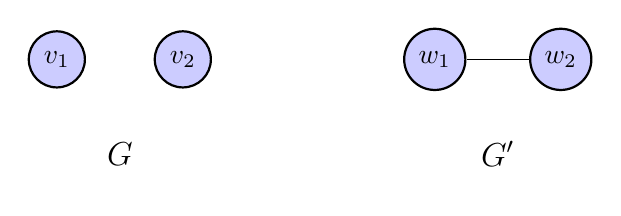
\begin{tikzpicture}  
      [scale=.8,auto=left,every node/.style={circle,fill=blue!20,draw=black,thick}]
      \node (n1) at (0,0) {$v_1$};
      \node (n2) at (2,0) {$v_2$};
      \node (n3) at (6,0) {$w_1$};
      \node (n4) at (8,0) {$w_2$};
      
      \foreach \from/\to in {n3/n4}
      \draw (\from) -- (\to);

      \node[draw=none, fill=none, font=\large] at (1,-1.5) {$G$};
      \node[draw=none, fill=none, font=\large] at (7,-1.5) {$G'$};
\end{tikzpicture}
}%
  \caption{$G$ y $G'$ no son isomorfos}
  \label{fig:homomorfo_no_isomorfo}
\end{figure}

   Sin embargo $\varphi$ no es un isomorfismo, pues $\left\lbrace \varphi(v_1),\varphi(v_2)\right\rbrace=\left\lbrace w_1,w_2\right\rbrace\in E(G')$ pero $\left\lbrace v_1,v_2\right\rbrace\notin E(G)$.
\end{Ejm}
Tenemos en cambio que si una función $\varphi$ es un homomorfismo biyectivo y su inversa $\varphi^{-1}$ es también un homomorfismo, entonces $\varphi$ sí es un isomorfismo. De hecho, esto caracteriza a los isomorfismos entre grafos, como muestra la siguiente proposición.\clearpage
\begin{Prop}
   Sean $G$ y $G'$ dos grafos y $\varphi:V(G)\to V(G')$ una función. Las siguientes afirmaciones son equivalentes:
   \begin{itemize}
      \item[1.] $\varphi$ es un homomorfismo biyectivo de $G$ en $G'$ y $\varphi^{-1}$ es un homomorfismo de $G'$ en $G$.
      \item[2.] $\varphi$ es un isomorfismo de $G$ en $G'$.
   \end{itemize}
\end{Prop}
\begin{proof}
   $1\Rightarrow 2$ : Supongamos que $\varphi$ es un homomorfismo biyectivo de $G$ en $G'$ y $\varphi^{-1}$ es un homomorfismo de $G'$ en $G$. Sean $u,v \in V(G)$. Si $\left\lbrace u,v\right\rbrace\in E(G)$, como $\varphi$ es un homomorfismo, $\left\lbrace \varphi(u),\varphi(v)\right\rbrace\in E(G')$. Si $\left\lbrace \varphi(u),\varphi(v)\right\rbrace\in E(G')$, como $\varphi^{-1}$ es un homomorfismo y $\varphi$ es biyectivo, entonces $\left\lbrace u,v\right\rbrace=\left\lbrace \varphi^{-1}(\varphi(u)),\varphi^{-1}(\varphi(v))\right\rbrace\in E(G)$. Por tanto $\varphi$ es un isomorfismo de $G$ en $G'$.\par
   $2\Rightarrow 1$ : Supongamos que $\varphi$ es un isomorfismo de $G$ en $G'$. Por definición de isomorfismo, $\varphi$ es biyectiva. Si $u,v\in V(G)$ son tales que $\left\lbrace u,v\right\rbrace\in E(G)$ entonces $\left\lbrace \varphi(u),\varphi(v)\right\rbrace\in E(G')$, y por tanto $\varphi$ es un homomorfismo de $G$ en $G'$. Supongamos que $x,y\in V(G')$ son tales que $\left\lbrace x,y\right\rbrace\in E(G')$. Como $\varphi$ es biyectiva, existen $w_x,w_y\in V(G)$ tales que $\varphi(w_x)=x$ y $\varphi(w_y)=y$, luego $\left\lbrace \varphi(w_x),\varphi(w_y)\right\rbrace\in E(G')$. Como $\varphi$ es un isomorfismo, se tiene $\left\lbrace \varphi^{-1}(x),\varphi^{-1}(y)\right\rbrace=\left\lbrace w_x,w_y\right\rbrace\in E(G)$. Por tanto $\varphi^{-1}$ es un homomorfismo de $G'$ en $G$.
\end{proof}
\begin{Def}
   Decimos que un grafo $G$ es \textbf{vértice transitivo} si para cualquier par de vértices $u,v\in V(G)$ existe un automorfismo de $G$ que envía $u$ a $v$.    
\end{Def}
\begin{Ejm}
   Para todo $n\in\mathbb{N}$ con $n\ge 3$ se tiene que $C^n$ es un grafo vértice transitivo. Podemos suponer que $V(C^n)$ es de la forma $\left\lbrace v_0,v_1, \dots, v_{n-1}\right\rbrace$ con $E(C^n)=\left\lbrace v_0v_1, v_1v_2, \dots ,v_{n-2}v_{n-1}, v_{n-1}v_0\right\rbrace$. Sean $v_i,v_j\in V(C^n)$ cualesquiera. La función $\varphi :V(C^n)\to V(C^n):v_k\mapsto v_{(k+j-i)\bmod n}$ para cada $k\in\left\lbrace 0,1,\dots ,n-1\right\rbrace$, es un automorfismo que envía $v_i$ a $v_j$. Si representamos a $C^n$ como en la \Cref{fig:ciclo_n}, podemos pensar en $\varphi$ como una función que ``rota'' al grafo en sentido horario hasta llevar al vértice $v_i$ a la posición del vértice $v_j$.\clearpage
   \begin{figure}[H]
\centering
\resizebox{0.35\textwidth}{!}{
   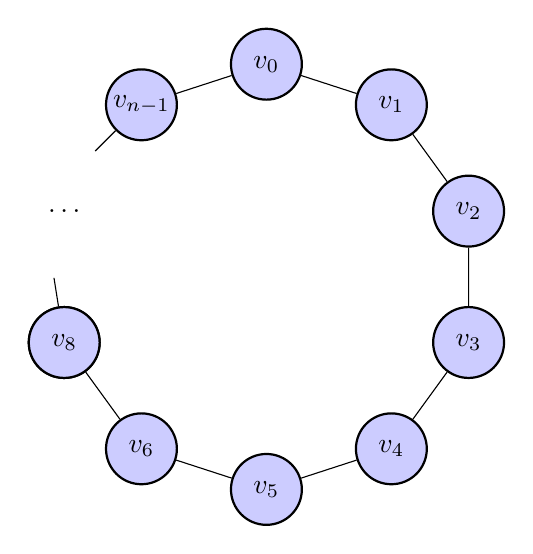
\begin{tikzpicture}[scale=0.9, auto=left, every node/.style={circle, fill=blue!20, draw=black, thick, inner sep=0pt, minimum size=0.9cm}]

     % Vértices visibles de v_0 a v_8 en sentido horario
     \node (v0) at (90:3) {$v_0$};
     \node (v1) at (54:3) {$v_1$};
     \node (v2) at (18:3) {$v_2$};
     \node (v3) at (-18:3) {$v_3$};
     \node (v4) at (-54:3) {$v_4$};
     \node (v5) at (-90:3) {$v_5$};
     \node (v6) at (-126:3) {$v_6$};
     \node (v7) at (-162:3) {$v_7$};
     \node (v8) at (198:3) {$v_8$};

     % Último vértice v_{n-1}
     \node (vn1) at (126:3) {$v_{n-1}$};

     % Vértices invisibles y puntos para la discontinuidad
     \node[draw=none, fill=none, minimum size=0pt] (v9_inv) at (180:3) {};
     \node[draw=none, fill=none, minimum size=0pt] (vn2_inv) at (144:3) {};
     \node[draw=none, fill=none, minimum size=0pt] (dots) at (162:3) {$\dots$};

     % Aristas continuas principales
     \draw (v0) -- (v1);
     \draw (v1) -- (v2);
     \draw (v2) -- (v3);
     \draw (v3) -- (v4);
     \draw (v4) -- (v5);
     \draw (v5) -- (v6);
     \draw (v6) -- (v7);
     \draw (v7) -- (v8);

     % Arista normal entre v_{n-1} y v_0
     \draw (vn1) -- (v0);

     % Aristas hacia/desde la zona discontinua
     \draw (v8) -- (v9_inv);
     \draw (vn2_inv) -- (vn1);

   \end{tikzpicture}}%
   \caption{El grafo $C^n$}
   \label{fig:ciclo_n}
\end{figure}

\end{Ejm}
